\documentclass{beamer}
\usepackage{amsfonts}
\usepackage{beamerprosper}
\usepackage{color}
\usepackage{lmodern} 
\usetheme{Hannover}
\title{Disease and Development: The Effect of Life Expectancy on Economic Growth}
\author{Daron Acemo\u{g}lu and Simon Johnson}
\institute{Dil\c{s}at Dalk{\i}ran-Ozel}
\date{\today}

\begin{document}

\begin{frame}
\titlepage
\end{frame}

\section{Outline} 
\begin{frame}
\frametitle{Outline} 
\begin{itemize}
\item The Paper: Motivation and Contribution
\item The Paper: Methodology
\item Replication Analysis
\item My Contribution
\end{itemize}
\end{frame}

\section{The Paper: Motivation and Contribution}
\begin{frame}
\frametitle{The Paper: Motivation and Contribution}
\begin{itemize}
\item Better health conditions $\rightarrow$ life expectancy
\item life expectancy $\xrightarrow{?}$ economic growth 
\item Acemo\u{g}lu and Johnson: Effect of life expectancy on economic growth between 1940-1980
\begin{itemize}
\item 1940-1980
\begin{itemize}
\item wave of global drug and chemical innovations
\item establishment of the World Health Organization
\item change in international values
\end{itemize}
\end{itemize}
\item Main Result: No evidence that increase in life expectancy have a remarkable effect on economic growth as all its effect is dominated mostly by population growth
\end{itemize}
\end{frame}

\section{The Paper: Methodology}
\begin{frame}
\frametitle{The Paper: Methodology}
\begin{Itemize}
\item Solow growth model with human capital
\item 1st Implication: Higher life expectancy $\rightarrow$ higher population $\rightarrow$ decrease per capita GDP 
\item 2nd Implication: Higher life expectancy $\rightarrow$ higher productivity $\rightarrow$ accumulation of capital $\rightarrow$ increase per capita GDP 
\begin{equation}
y_{it}=\pi x_{it}+ \gamma_{i} + \mu_{t} + Z'_{it}\beta + \epsilon_{it} \nonumber
\end{equation}
\end{Itemize}
\end{frame}

\begin{frame}
\frametitle{The Paper: Methodology}
\begin{equation}
y_{it}=\pi x_{it}+ \gamma_{i} + \mu_{t} + Z'_{it}\beta + \epsilon_{it}
\end{equation}
\begin{Itemize}
\item y is log income per capita
\item x is log life expectancy at birth
\item $\pi$ is the parameter of interest
\item $\gamma$ is fixed effect which is a function of the parameters: $A_{i}$, TFP, $h_{i}$, human capital, $N_{i}$,total population (and employment)
\item $\mu_{t}$ is time varying factors common across all countries
\item $Z_{it}$ is vector of other control variables
\item Data: 75 countries from Western Europe, Oceania, the Americas and Asia between 1940 and 1980 (or 2000). Most of the data is collected from UN Demographic Yearbooks and League of Nations.
\end{Itemize}
\end{frame}

\section{Replication Analysis} 
\begin{frame}
\frametitle{Replication Analysis} 
\begin{itemize}
\item OLS and 2SLS
\item OLS: biased, inconsistent due to omitted variable and reverse causality
\end{itemize}
\begin{center}
\begin{figure}
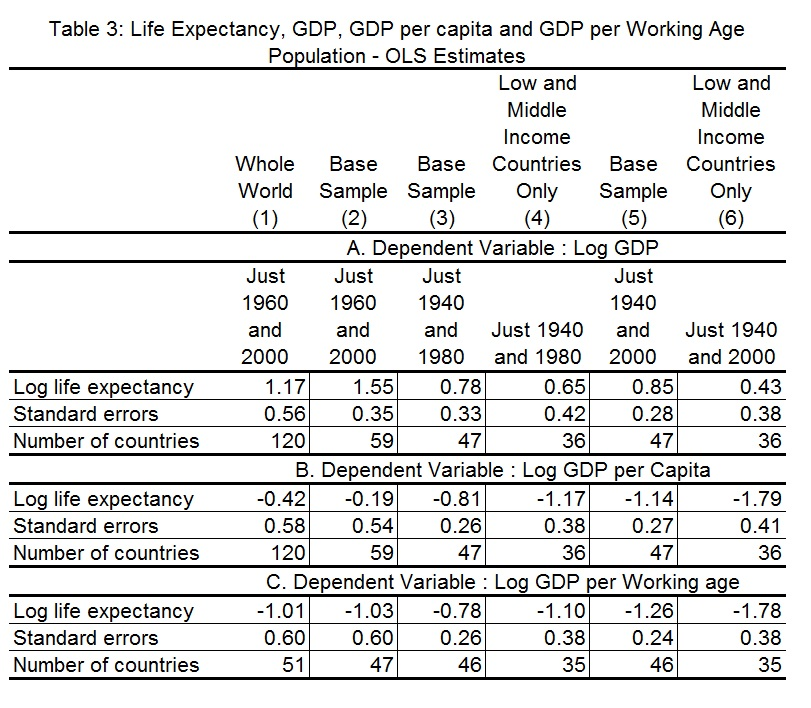
\includegraphics[height=2.5in]{table3}
\end{figure}
\end{center}
\end{frame}

\begin{frame}
\frametitle{Replication Analysis} 
\begin{itemize}
\item 2SLS : unbiased, consistent
\item Predicted Mortality instrument for life expectancy 
\begin{equation}
M^{l}_{it} = \sum\limits_{d \in D} [(1-I_{dt})M_{di40}+I_{dt}M_{dFt}]
\end{equation}
\item $M^{l}_{it}$ : Predicted mortality
\item $I_{dt}$: dummy for intervention for disease d at time t
\item $M_{di40}$: Pre-intervention mortality (pre 1940)
\item $M_{dFt}$: Mortality rate from disease d at the health frontier
\end{itemize}
\end{frame}

\begin{frame}
\frametitle{Replication Analysis} 
Results:
\begin{itemize}
\item positive relation between life expectancy and population growth
\item slight positive relationship between log GDP and log life expectancy
\item negative relationship between GDP per capita and log life expectancy
\item No evidence on large increase in life expectancy lead to significant increase in per capita GDP
\end{itemize}
\end{frame}

\section{My Contribution} 
\begin{frame}
\frametitle{My Contribution} 
\begin{itemize}
\item So far: Replication analysis and generate an index for armed conflict (ongoing)
\item Introducing a new instrument : Armed conflict
\item Armed conflict may destroy physical and human capital $\rightarrow$ validity?
\item Hence; Sargan test for validity
\item If not, 
\begin{itemize}
\item continue with the same instrument
\item find another instrument: investment on long term contracts ?
\end{itemize}
\end{itemize}
\end{frame}

\end{document}
